\lstset{
  basicstyle=\fontsize{11}{15}\selectfont\ttfamily
}
\section{Datenmodell}
\subsection{OEBBError}
Ein Fehler beschreibt den Zustand einer Funktion, sollte diese einen gewissen Grenzwert über- oder unterschreiten.

\begin{lstlisting}[language=Typescript, caption={OEBB-Error}]
export class OEBBError{
  constructor(
    public name: String,
    public date: String,
    public zustand: String
  ){}
}
\end{lstlisting}

\subsection{OEBBFunktion}
Eine Funktion ist jeweils eine spezifische Messung, welche in den QTX-Dateien abgespeichert ist.

\begin{lstlisting}[language=Typescript, caption={OEBB-Funktion}]
export class OEBBFunktion{
  constructor(
    public id: number,
    public beschreibung: string,
    public headersize: number,
    public entries: number,
    public echtEntries: number,
    public numRead: number,
    public messergebnisse: OEBBMessergebnisse[]
  ){}
}
\end{lstlisting}

\subsection{OEBBKriterien}\label{OEBBKriterien}
Die Kriterien sind über den Zustand verschiedenen Funktionen zugeordnet und bilden die Werte, welche nicht über- oder unterschritten 
werden dürfen.

\begin{lstlisting}[language=Typescript, caption={OEBB-Kriterien}]
export class OEBBKriterien{
  constructor(
    public name: string,
    public angesprochen: number,
    public minWert: number,
    public maxWert: number,
    public istWert: number,
    public resultCode: number,
    public maskMin: number,
    public maskMax: number,
    public messCount: number
  ){}
}
\end{lstlisting}

\subsection{OEBBMessergebenisse}
Die Messergebnisse sind die spezifischen Messungen, welche jeweils zu einer Funktion zugeordnet sind. 

\begin{lstlisting}[language=Typescript, caption={OEBB-Messergebnisse}]
export class OEBBMessergebnisse{
  constructor(
    public id: number,
    public number: number,
    public yWert: number,
    public mittel: number,
    public max: number,
    public min: number
  ){}
}
\end{lstlisting}

\section{Service} \label{service}
Hier werden die Funktionen und Kriterien der verschiedenen QTX-Dateien gespeichert, um sie dem Rest der Anwendung zur Verfügung zu 
stellen. Über die Hilfsmethoden \lstinline | setFunctions | und \lstinline | setKriterien | werden die Daten im Service gespeichert
und mit den Hilfsmethoden \lstinline | getFunctions | und \lstinline | getKriterien | können die Daten wieder abgerufen werden.

\begin{lstlisting}[language=Typescript, caption={OEBB-Service}]
export class OebbService {
  private functions: OEBBFunktion[];
  private kriterien: OEBBKriterien[];

  constructor() {
    this.functions = [];
    this.kriterien = [];
  }
  setFunctions(data: OEBBFunktion[]){
    this.functions = data;
  }
  getFunctions(){
    return this.functions;
  }
  setKriterien(data: OEBBKriterien[]){
    this.kriterien = data;
  }
  getKriterien(){
    return this.kriterien;
  }
}
\end{lstlisting}

\section{Auswählen der Datei} \label{auswahlkomponente}
Hier wird die Datei ausgewählt, welche in der Visualisierungs-Komponenete angezeigt werden soll. Zuerst wurde versucht, die Datei 
über einen file-input auszuwählen und den Namen dieser Datei dann über einen HTTP-Request an das Backend zu schicken, wo die Daten
dieser Datei ausgewertet und in Funktionen und Kriterien aufgeteilt zurückgeschickt werden. 

\begin{lstlisting}[language=HTML, caption={Fileinput}]
    <input type="file" class="file-input" (change)="onFileSelected($event)">
\end{lstlisting}

Dieser Fileinput öffnet ein Explorer-Fenster, wo dann die Datei ausgewählt werden kann.

\begin{figure}[H]
    \centering
    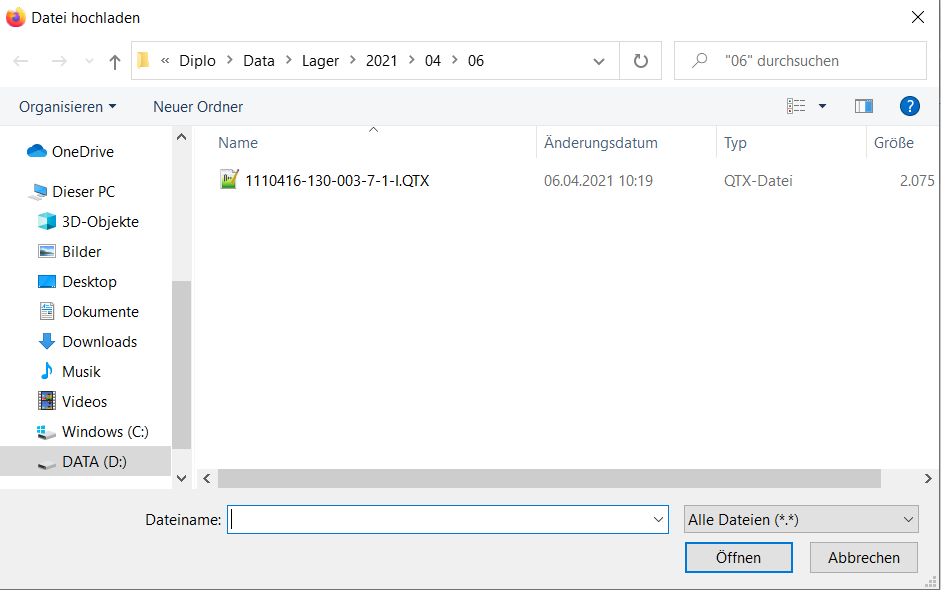
\includegraphics[width=0.80\textwidth]{pics/filexplorer.PNG}
    \caption{File-Explorer}
    \label{fig:fileexplorer}
\end{figure}

Da die Dateien, mit denen gearbeitet wird, häufig über die verschiedenen Zustände hinweg oft die gleichen Namen haben und das nicht 
aus den Dateien selbst herauslesbar ist, wurde als Lösung eine Funktion implementiert, mit welcher vor dem Fileinput ein Zustand 
ausgewählt wird.

Mögliche Zustände:
\begin{itemize}
    \item Auslauf / Auslauf 2: Hier wird getestet, wie sich der Antrieb beim Auslaufen lassen verhält
    \item Lager: Hier wird das Radwellenlager, das Bremswellenlager und das Motorwellenlager des Antriebs getestet
    \item Schlag: Hier wird gemessen, ob der Antrieb rund läuft
    \item Warmlauf: Ein Testlauf nachdem der Antrieb warmgelaufen ist
    \item Wuchtlauf: Hier wird der Antrieb auf die Unwucht gemessen
\end{itemize}

\begin{lstlisting}[language=HTML, caption={Checkboxen zum Auswählen des Zustandes}]
<section class="example-section">
  <mat-checkbox class="example-margin" [disabled]="disabled" (change)="onAuslaufSelected()">Auslauf</mat-checkbox>&nbsp;&nbsp;
  <mat-checkbox class="example-margin" [disabled]="disabled" (change)="onAuslauf2Selected()">Auslauf 2</mat-checkbox>&nbsp;&nbsp;
  <mat-checkbox class="example-margin" [disabled]="disabled" (change)="onLagerSelected()">Lager</mat-checkbox>&nbsp;&nbsp;
  <mat-checkbox class="example-margin" [disabled]="disabled" (change)="onSchlagSelected()">Schlag</mat-checkbox>&nbsp;&nbsp;
  <mat-checkbox class="example-margin" [disabled]="disabled" (change)="onWarmSelected()">Warmlauf</mat-checkbox>&nbsp;&nbsp;
  <mat-checkbox class="example-margin" [disabled]="disabled" (change)="onWuchtSelected()">Wuchtlauf</mat-checkbox>
</section>
\end{lstlisting}

Danach wurde der Request erweitert, um neben dem Dateinamen auch den ausgewählten Zustand als Parameter mitzuschicken.

\begin{lstlisting}[language=Typescript, caption={Http-Request für Funktionen und Kriterien}]
    const file: File = event.target.files[0];

    const f : OEBBFunktion[] = await this.httpClient
      .get<OEBBFunktion[]>('https://localhost:5001/' + this.zustand + '/' + file.name)
      .toPromise();
    const k : OEBBKriterien[] = await this.httpClient
      .get<OEBBKriterien[]>('https://localhost:5001/criteria/' + this.zustand + '/' + file.name)
      .toPromise();

    this.service.setFunctions(f);
    this.service.setKriterien(k);
\end{lstlisting}

Die Funktionen und Kriterien, die der HTTP-Request zurückliefert, werden in dem Service gespeichert, sodass im Rest der Anwendung
darauf zugegriffen werden kann [\ref{service}].

In den verschiedenen \lstinline | onZustandSelected | Methoden wird jeweils der ausgewählte Zustand
gesetzt und die Checkboxen deaktiviert, um immer nur einen Zustand auswählen zu können.

\begin{lstlisting}[language=Typescript, caption={Eine der onZustandSelect-Methoden}]
    onAuslaufSelected(): void {
    this.disabled = true;
    this.zustand = 'Auslauf';
  }
\end{lstlisting}

Die Weiterleitung auf die Visualisierungskomponente wird über ein Switch-Case-Statement durchgeführt. Je nach Anzahl der Kriterien, 
die vom Backend zurückgeschickt werden, wird der Benutzer auf die richtige Komponente weitergeleitet. Die Weiterleitung selbst
passiert über einen Router, welcher die verschiedenen Komponenten miteinander verbindet. 

\begin{lstlisting}[language=Typescript, caption={Switch-Case für die Weiterleitung zur Visualisierung}]
    switch(k.length){
      case 27:
        this.router.navigate(['show-function']);
        break;
      case 2:
        this.router.navigate(['show-function-auslauf']);
        break;
      case 15:
        this.router.navigate(['show-function-schlaglauf']);
        break;
      case 8:
        this.router.navigate(['show-function-warmlauf']);
        break;
      case 7:
        this.router.navigate(['show-function-wuchtlauf']);
        break;
    }
\end{lstlisting}

Die fertige Komponente für das Auswählen der Datei sieht folgendermaßen aus (\ref{fig:dateiauswählen}):

\begin{figure}[H]
    \centering
    \includegraphics[width=0.80\textwidth]{pics/choosefileausgewählt.PNG}
    \caption{Fertige Komponente zum Dateien auswählen}
    \label{fig:dateiauswählen}
\end{figure}

Hier wurde bereits der Zustand \dq Lager\dq  ausgewählt, folgendermaßen wird nun eine Lagerdatei aus dem Explorer ausgewählt und der 
Benutzer wird auf die Visualisierungskomponente des Lagerzustandes weitergeleitet.

\section{Visualisierungskomponente} \label{visualisation}
Hier werden die Funktionen der Datei visualisiert, welche zuvor in der Auswahlskomponente [\ref{auswahlkomponente}] ausgewählt wurde.
Zur Visualisierung selbst wird die JavaScript-Bibliothek ng2-charts benutzt, welche auf der chart.js-Bibliothek 
basiert. 

\subsection{Initialisierung}
Beim Initialisieren der Komponente werden zuerst die Funktionen und Kriterien aus dem Service geladen, um sie innerhalb der 
Komponente nur einmal aus dem Service abrufen zu müssen.

\begin{lstlisting}[language=Typescript, caption={Initialisierung der Komponente}]
  async ngOnInit(): Promise<void> {
    this.functions = this.service.getFunctions();
    this.kriterien = this.service.getKriterien();
  }
\end{lstlisting}

Danach werden die Grundoptionen des Diagramms gesetzt, wo später die Daten dargestellt werden.

\begin{lstlisting}[language=Typescript, caption={Grundoptionen des Diagramms}]
  dataPoints: ChartDataSets[] = [];
  labels: Label[] = [];
  options = {
    responsive: false,
    scales:  {
    }
  };
  colors: Color[] = [
    {
      borderColor: 'black',
      backgroundColor: undefined
    },
  ];
  legend = true;
  plugins = [];
  type: ChartType = 'line';
\end{lstlisting}

Die dataPoints sind die Punkte, wodurch das Diagramm aufgebaut wird. Da zum Initialisierungszeitpunkt noch keine Daten vorhanden sind,
bleiben diese vorerst leer, ebenso wie die labels, welche die Namen der verschiedenen Graphen darstellen. Beide werden später in einer
eigenen Methode befüllt. Mit \lstinline | options responsive: false | wird das Verhalten der Größenänderung bei verschiedenen
Fenstergrößen ausgestellt. Da diese Anwendung nur auf dem immer gleichen Rechner laufen muss, ist diese Option in diesem Fall unnötig.
Mit \lstinline | borderColour: 'black' | wird die Farbe des Graphengerüsts auf schwarz gestellt und mit \lstinline | backgroundColour: 'undefined' | 
wird die Farbe, mit der die Graphen normalerweise hinterlegt werden, ausgestellt. \lstinline | legend = true | bedeutet,
dass die DataSets, welche in dem Graph benutzt werden, angezeigt werden. Mit \lstinline | type: ChartType = 'line' | wird dem 
Diagramm mitgeteilt, welche Art von Diagramm es ist, in diesem Fall ein Linien-Diagramm.

Der HTML-Code des Diagramms sieht folgendermaßen aus:

\begin{lstlisting}[language=HTML, caption={HTML für das Diagramm}]
<div id="one" class="chartjs-block">
  <canvas baseChart height="600" width="1500"
      [datasets]="dataPoints"
      [labels]="labels"
      [options]="options"
      [colors]="colors"
      [legend]="legend"
      [chartType]="type"
      [plugins]="plugins">
  </canvas>
</div>
\end{lstlisting}

\subsection{Auswählen der Funktion}
In einem Dropdown-Menü kann die gewünschte Funktion ausgewählt werden, welche der Benutzer sich ansehen möchte. Sobald eine Funktion
ausgewählt wurde, wird die Methode \lstinline | onSelect | aufgerufen, welche die Visualisierung durchführt.

\begin{lstlisting}[language=HTML, caption={Dropdown-Menü für die Funktionen}]
<div id="select">
  <mat-form-field appearance="fill" (change)="onSelect()">
    <select matNativeControl [(ngModel)]="selectedFunction" name="f">
      <option value="" selected></option>
      <option *ngFor="let f of functions" [value]="f.beschreibung">{{f.beschreibung}}</option>
    </select>
  </mat-form-field>
</div>
\end{lstlisting}

\subsection{Darstellen der Funktion}
Wie bereits beschrieben wird zur Darstellung der Daten ng2-charts benutzt und die Visualisierung wird in der Methode
\lstinline | onSelect | durchgeführt, welche in drei Teile aufgeteilt werden kann.

\subsubsection{Reset und Kriterien}
Zuerst werden alle Daten und Kriterien gelöscht, um sicherzustellen, dass keine falschen Daten oder Kriterien von einem vorherigen 
Aufruf der Methode noch vorhanden sind.

\begin{lstlisting}[language=Typescript, caption={Zurücksetzen der Daten}]
    this.disabled = false;
    this.dataMittel = [];
    this.dataMax = [];
    this.dataMin = [];
    this.labels = [];
    this.kriteriumOneMin = [];
    this.kriteriumOneMax = [];
    this.kriterium = [];
    this.kriteriumTwoMin = [];
    this.kriteriumTwoMax = [];
    this.kriteriumThreeMin = [];
    this.kriteriumThreeMax = [];
    this.pushCount = 50;
\end{lstlisting}

Danach werden die richtigen Kriterien aus der Liste der Kriterien, die von dem Backend kommt, herausgelesen. Da in einer Datei mehrere
Funktionen sind und diese nicht alle die gleichen Kriterien haben, sind in der Datei alle Kriterien zusammengefasst gespeichert. Die 
richtigen Kriterien werden über den Namen der Funktion herausgefiltert und in ein extriges Array von Kriterien gespeichert. Sollte 
der Name der ausgewählten Funktion auf keinen der Fälle zutreffen, werden in der Graphik keine Kriterien angezeigt. Dies wird zum 
Beispiel bei den Spektrums-Funktionen genutzt, da diese keine Kriterien benötigen (\ref{fig:graphwok}).

\begin{lstlisting}[language=Typescript, caption={Filtern der Kriterien}]
    switch(f.beschreibung){
      case 'LagerEnvelope(Bremswelle A)':
        this.kriterium = [this.kriterien[1], this.kriterien[9], this.kriterien[19]];
        break;
      case 'LagerEnvelope(Bremswelle B)':
        this.kriterium = [this.kriterien[5], this.kriterien[13], this.kriterien[23]];
        break;
      case 'LagerEnvelope(Motorwelle A)':
        this.kriterium = [this.kriterien[2], this.kriterien[10], this.kriterien[20]];
        break;
      case 'LagerEnvelope(Motorwelle B)':
        this.kriterium = [this.kriterien[6], this.kriterien[14], this.kriterien[24]];
        break;
      case 'LagerEnvelope(Radwelle A)':
        this.kriterium = [this.kriterien[3], this.kriterien[11], this.kriterien[21]];
        break;
      case 'LagerEnvelope(Radwelle B)':
        this.kriterium = [this.kriterien[7], this.kriterien[15], this.kriterien[25]];
        break;
      default:
        this.kriterium = [];
        break;
    }
\end{lstlisting}

\subsubsection{Befüllen der Daten}
\begin{lstlisting}[language=Typescript, caption={Befüllen der Daten}]
    if(this.kriterium.length > 0){
      for(let i = 0; i < 100; i++){
        this.dataMittel.push(f.messergebnisse[i].mittel);
        this.dataMax.push(f.messergebnisse[i].max);
        this.dataMin.push(f.messergebnisse[i].min);
        this.labels.push(f.messergebnisse[i].yWert.toString());
        this.kriteriumOneMin.push(this.kriterium[0].minWert);
        this.kriteriumOneMax.push(this.kriterium[0].maxWert);
        this.kriteriumTwoMin.push(this.kriterium[1].minWert);
        this.kriteriumTwoMax.push(this.kriterium[1].maxWert);
        this.kriteriumThreeMin.push(this.kriterium[2].minWert);
        this.kriteriumThreeMax.push(this.kriterium[2].maxWert);
      }
    }
    else{
      for(let i = 0; i < 100; i++){
        console.log(f.messergebnisse)
        this.dataMittel.push(f.messergebnisse[i].mittel);
        this.dataMax.push(f.messergebnisse[i].max);
        this.dataMin.push(f.messergebnisse[i].min);
        this.labels.push(f.messergebnisse[i].yWert.toString());
      }
    }
\end{lstlisting}

Hier werden die jeweils ersten hundert Messergebnisse für den Mittelwert, den Maximalwert und den Minimalwert in die dafür vorgesehenen
Hilfsarrays gefüllt. Sollte es sich bei der ausgewählten Funktion um eine jener Funktionen handeln, welche Kriterien benötigt, werden 
diese ebenfalls in die dafür vorgesehenen Hilfsarrays gefüllt.

\subsubsection{Zeichnen der Graphik}
Um die Graphik zeichnen zu können, müssen hier die dataPoints befüllt werden. 

\begin{lstlisting}[language=Typescript, caption={Befüllen der DataPoints}]
    if(this.kriterium.length > 0){
      this.dataPoints = [
        {fill: false, data: this.kriteriumOneMin, label: this.kriterium[0].name + " Min"},
        {fill: false, data: this.kriteriumOneMax, label: this.kriterium[0].name + " Max"},
        {fill: false, data: this.kriteriumTwoMin, label: this.kriterium[1].name + " Min"},
        {fill: false, data: this.kriteriumTwoMax, label: this.kriterium[1].name + " Max"},
        {fill: false, data: this.kriteriumThreeMin, label: this.kriterium[2].name + " Min"},
        {fill: false, data: this.kriteriumThreeMax, label: this.kriterium[2].name + " Max"},
        {fill: false, data: this.dataMittel, label: f.beschreibung + " Mittel"},
        {fill: false, data: this.dataMax, label: f.beschreibung + " Max"},
        {fill: false, data: this.dataMin, label: f.beschreibung + " Min"}
      ]
    }
    else{
      this.dataPoints = [
        {fill: false, data: this.dataMittel, label: f.beschreibung + " Mittel"},
        {fill: false, data: this.dataMax, label: f.beschreibung + " Max"},
        {fill: false, data: this.dataMin, label: f.beschreibung + " Min"}
      ]
    }
\end{lstlisting}

Die dataPoints sind ein Array von ChartDataSets und bestehen jeweils aus fill, data und label. Fill wird benutzt, um dem Graph zu sagen,
ob er den Bereich unter dem Graphen einfärben soll, in diesem Fall wird dieser Bereich nicht eingefärbt. Data sind die jeweiligen Werte,
aus denen der Graph gebildet wird und Label ist der Name des jeweiligen Graphen. Auch hier wird wieder unterschieden zwischen einer 
Funktion mit Kriterien und einer Funktion ohne Kriterien. Sollte die ausgewählte Funktion Kriterien besitzten, werden diese ebenfalls in
dem Diagramm eingezeichnet.

\begin{figure}[H]
    \centering
    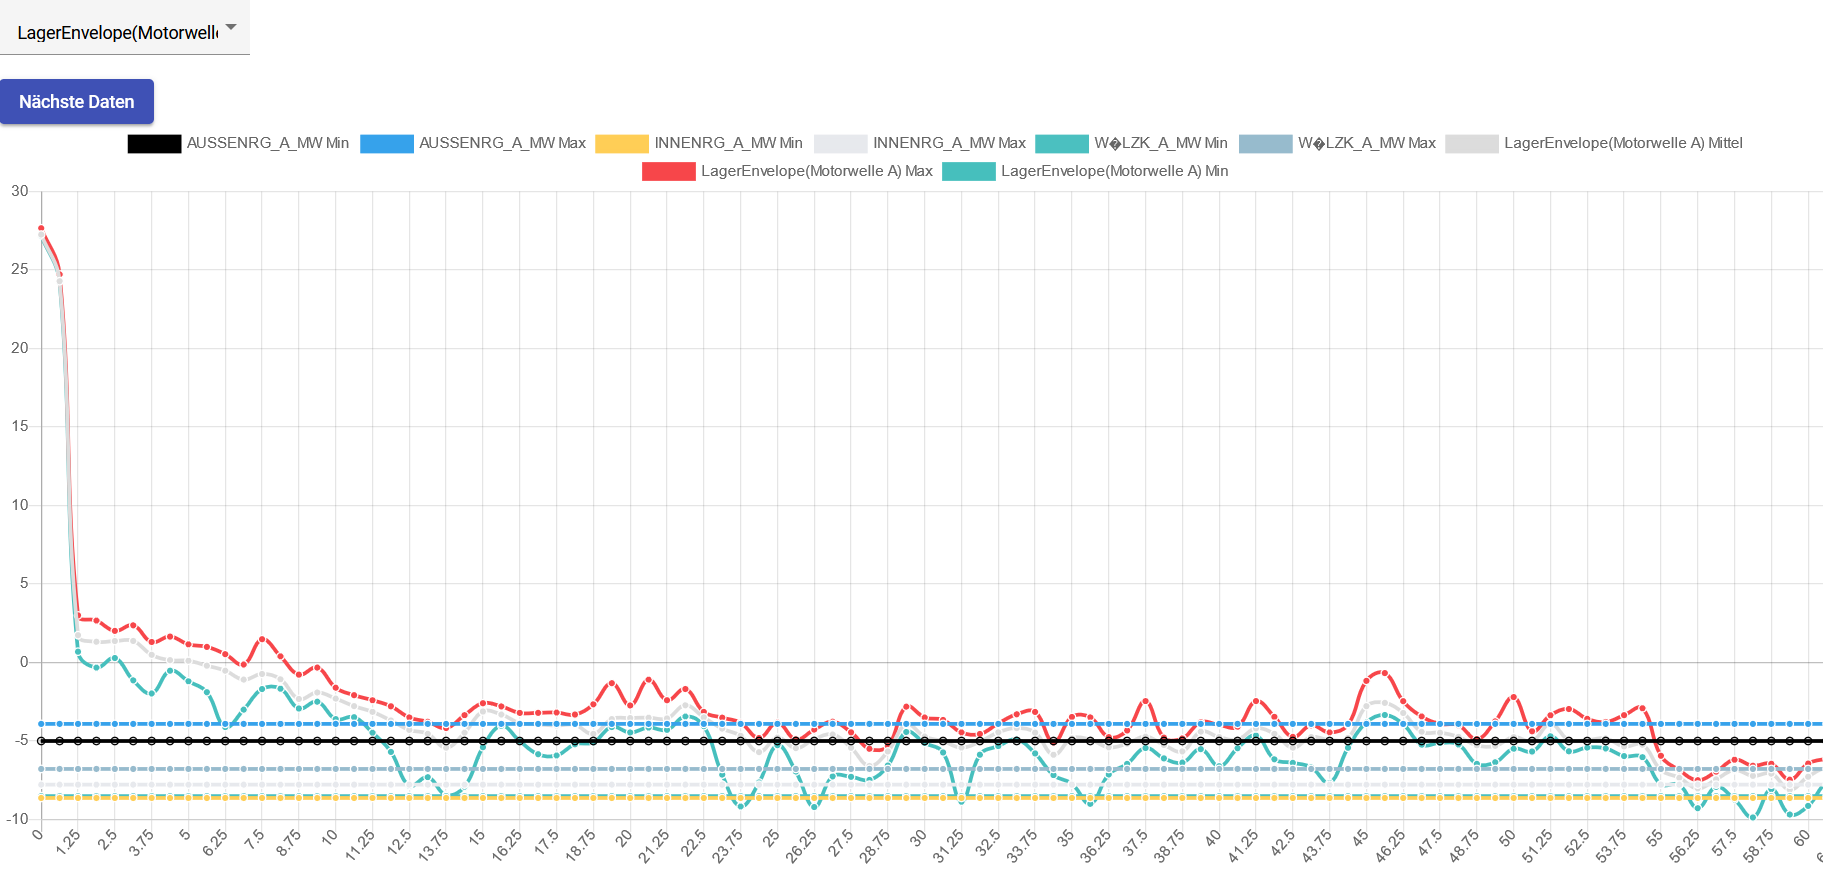
\includegraphics[width=0.80\textwidth]{pics/graphwk.PNG}
    \caption{Beispiel einer Funktion mit Kriterien}
    \label{fig:graphwk}
\end{figure}

\begin{figure}[H]
    \centering
    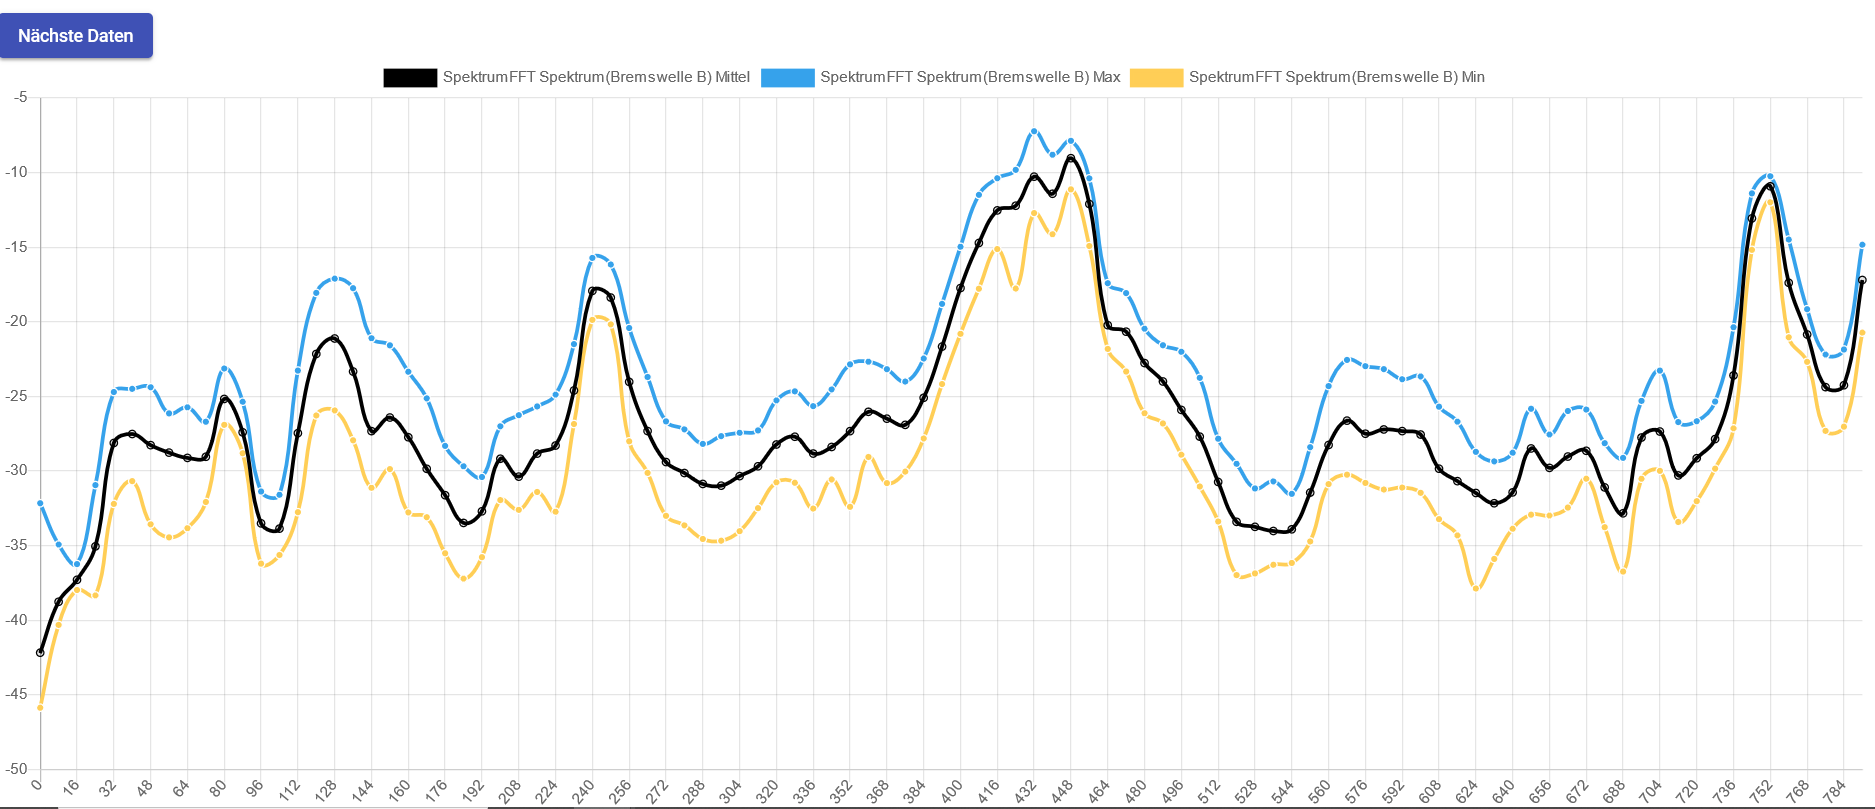
\includegraphics[width=0.80\textwidth]{pics/graphwok.PNG}
    \caption{Beispiel einer Funktion ohne Kriterien}
    \label{fig:graphwok}
\end{figure}

\subsection{Push}
Viele der Funktionen, die dargestellt werden, haben zu viele Messergebnisse und daher auch dataPoints, um sie übersichtlich in einem
Diagramm darstellen zu können. Daher werden zuerst, wie oben beschrieben, nur die ersten hundert Werte geladen und über die folgende
Methode push werden immer die nächsten 50 Werte angezeigt. 

\begin{lstlisting}[language=Typescript, caption={Push-Methode}]
  public push(): void {
    this.dataMittel = [];
    this.dataMax = [];
    this.dataMin = [];
    this.labels = [];
    let f: OEBBFunktion = new OEBBFunktion(0,'',0,0,0,0,this.messergebnisse);
    this.functions.forEach(element => {if(element.beschreibung === this.selectedFunction){f = element;}});
    if(f.messergebnisse[this.pushCount+50] === undefined){
      this.disabled = true;
    }
    for(let i = this.pushCount - 50; i < this.pushCount + 50; i++){
      this.dataMittel.push(f.messergebnisse[i].mittel);
      this.dataMax.push(f.messergebnisse[i].max);
      this.dataMin.push(f.messergebnisse[i].min);
      this.labels.push(f.messergebnisse[i].yWert.toString());
    }

    if(this.kriterium.length > 0){
      this.dataPoints = [
        {fill: false, data: this.kriteriumOneMin, label: this.kriterium[0].name + " Min"},
        {fill: false, data: this.kriteriumOneMax, label: this.kriterium[0].name + " Max"},
        {fill: false, data: this.kriteriumTwoMin, label: this.kriterium[1].name + " Min"},
        {fill: false, data: this.kriteriumTwoMax, label: this.kriterium[1].name + " Max"},
        {fill: false, data: this.kriteriumThreeMin, label: this.kriterium[2].name + " Min"},
        {fill: false, data: this.kriteriumThreeMax, label: this.kriterium[2].name + " Max"},
        {fill: false, data: this.dataMittel, label: f.beschreibung + " Mittel"},
        {fill: false, data: this.dataMax, label: f.beschreibung + " Max"},
        {fill: false, data: this.dataMin, label: f.beschreibung + " Min"}
      ]
    } else{
      this.dataPoints = [
        {fill: false, data: this.dataMittel, label: f.beschreibung + " Mittel"},
        {fill: false, data: this.dataMax, label: f.beschreibung + " Max"},
        {fill: false, data: this.dataMin, label: f.beschreibung + " Min"}
      ]
    }
    this.pushCount += 50;
  }
\end{lstlisting}

Zuerst werden die dataPoints zurückgesetzt, um Platz für die neuen Werte zu schaffen. Da die Kriterien jeweils statische Werte sind,
müssen diese nicht zurückgesetzt werden. Danach wird überprüft, ob es nach den derzeitigen Werten noch Werte gibt, sollte dies nicht
der Fall sein, wird der Button, mit dem die Daten weitergeschaltet werden, deaktiviert. Dann werden die neuen Werte wieder in ihre 
jeweiligen Hilfsarrays gespeichert, ähnlich wie beim ersten Befüllen der Daten. Der pushCount ist hierbei ein Laufwert, über den die 
derzeitigen und nächsten Daten verwaltet werden. Hiernach werden die Daten wieder neu in die dataPoints gefüllt und der Graph neu 
gezeichnet. 

\section{Auswertungskomponente}
Hier können alle Fehler nach Zustand, Jahr, Monat und Tag gefiltert und ausgegeben werden. 

\subsection{Auswahl der Kriterien}
Die Kriterien, welche wie oben beschrieben aus Zustand, Jahr, Monat und Tag bestehen, werden jeweils einzeln aus den dafür vorgesehenen
Dropdown-Menüs ausgewählt (\ref{fig:auswahl}) und über Objekt-Binding in die Komponente übertragen. Das \lstinline|[(ngModel)]="selectedZustand"|
referenziert auf das gleichnamige Objekt in der Typescript-Datei.
\begin{figure}[H]
    \centering
    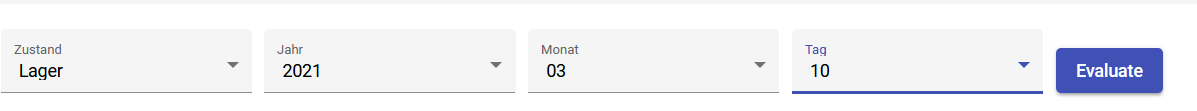
\includegraphics[width=0.80\textwidth]{pics/dropdown.PNG}
    \caption{Kriterienauswahl}
    \label{fig:auswahl}
\end{figure}

\begin{lstlisting}[language=HTML, caption={HTML-Code des Dropdown-Menüs des Zustandes}]
  <mat-form-field appearance="fill">
    <mat-label>Zustand</mat-label>
    <select matNativeControl [(ngModel)]="selectedZustand" name="z">
        <option value="" selected></option>
        <option *ngFor="let z of zustand" [value]="z">{{z}}</option>
    </select>
  </mat-form-field>
\end{lstlisting}
\begin{lstlisting}[language=Typescript, caption={Binding-Objekte in der Typescript-Datei}]
  selectedYear = null;
  selectedMonth = null;
  selectedDay = null;
\end{lstlisting}

Es kann eine beliebige Kombination aus Kriterien ausgewählt werden, beispielsweise Zustand und Jahr, nur der Zustand oder alle vier 
Kriterien gleichzeitig. Sofern zu den ausgewählten Kriterien Fehler vorhanden sind, werden diese in einer Tabelle angezeigt, sollten 
keine Fehler vorhanden sein, wird eine Fehlernachricht ausgegeben.
\begin{figure}[H]
    \centering
    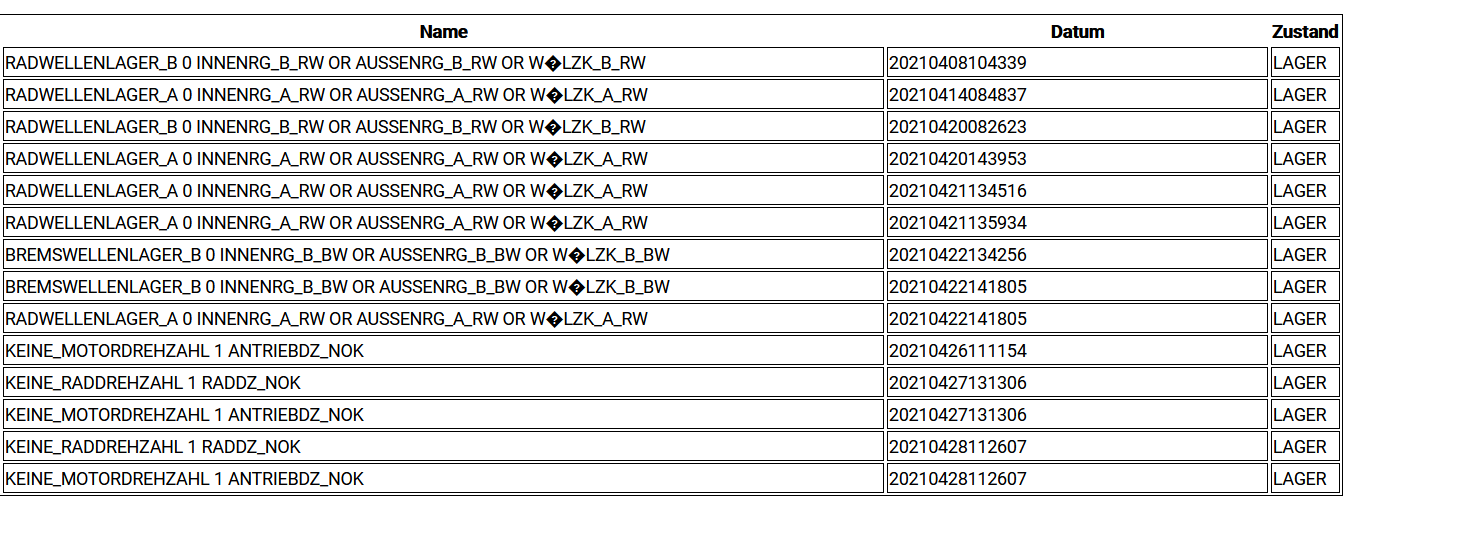
\includegraphics[width=0.80\textwidth]{pics/errors.PNG}
    \caption{Fehler gefiltert nach Kriterien}
    \label{fig:errors}
\end{figure}
\begin{figure}[H]
    \centering
    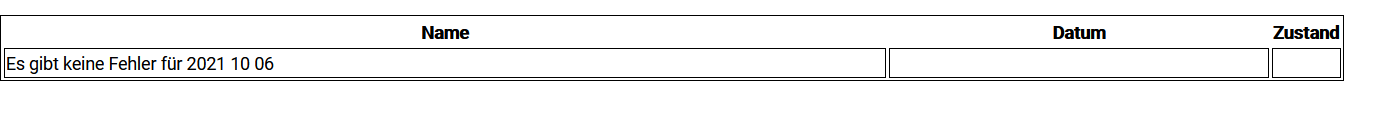
\includegraphics[width=0.80\textwidth]{pics/noerror.PNG}
    \caption{Keine Fehler für die ausgewählten Kriterien}
    \label{fig:noerrors}
\end{figure}

Die Tabelle, in der die Fehler ausgegeben werden, ist eine einfache HTML-Tabelle ohne TypeScript oder JavaScript. Über Objekt-Binding 
wird ein Objekt mit dem Namen errors in die Tabelle übergeben, welches mit einer einfachen ngFor durchiteriert und jeder einzelne Fehler
im Objekt angezeigt wird.

\begin{lstlisting}[language=HTML, caption={HTML-Code der Fehlertabelle}]
<table>
  <tr>
    <th>Name</th>
    <th>Datum</th>
    <th>Zustand</th>
  </tr>
  <tr *ngFor="let e of errors">
    <td>{{e.name}}</td>
    <td>{{e.date}}</td>
    <td>{{e.zustand}}</td>
  </tr>
</table>
\end{lstlisting}

\subsection{Mocking der Auswertungskomponente}
Für Testzwecke wurden die gesamten Daten der Auswertungskomponente zuerst gemockt, um Fehler im Produktivbetrieb zu minimieren.
Das Mocking selbst läuft über den ErrorMockingService, in welchem einige Fehler hartgecodet wurden.

\begin{lstlisting}[language=Typescript, caption={Error-Mocking-Service}]
export class ErrorMockingService {
  private errors: OEBBError[];

  constructor() {
    this.errors = [
      {name: 'RADWELLENLAGER_B	0	INNENRG_B_RW OR AUSSENRG_B_RW OR WAELZK_B_RW', date: '2021-04-20', zustand: 'Lager'},
      {name: 'RADWELLENLAGER_B	0	INNENRG_B_RW OR AUSSENRG_B_RW OR WAELZK_B_RW', date: '2021-05-17', zustand: 'Lager'},
      {name: 'UNWUCHT_A_RW	0	UNWUCHT_VA', date: '2021-07-12', zustand: 'Auslauf'},
      {name: 'MOTORWELLENLAGER_B	0	INNENRG_B_MW OR AUSSENRG_B_MW OR WAELZK_B_MW', date: '2021-04-19', zustand: 'Auslauf 2'},
      {name: 'RAD_A	0	PLANLAUF_A_MAX OR RUNDLAUF_A_MAX', date: '2021-03-01', zustand: 'Schlag'},
      {name: 'BREMSWELLENLAGER_B	0	INNENRG_B_BW OR AUSSENRG_B_BW OR WAELZK_B_BW', date: '2021-06-09', zustand: 'Warmlauf'},
      {name: 'BREMSWELLENLAGER_A	0	INNENRG_A_BW OR AUSSENRG_A_BW OR WAELZK_A_BW', date: '2021-05-25', zustand: 'Wuchtlauf'},
    ];
  }

  getErrors(zustandParam: String, dateParam?: String){
    if(dateParam == undefined){
      return this.errors.filter(x => x.zustand == zustandParam);
    }
    return this.errors.filter(x => x.zustand == zustandParam && x.date == dateParam)
  }
}
\end{lstlisting}

Zuerst wird ein Array aus OEBBErrors angelegt, welches im Konstruktor befüllt wird. Die Funktionsnamen und Zustände wurden hierfür aus
dem Produktivbetrieb ausgewählt, die Daten wurden zufällig zugeteilt. In der Funktion \lstinline | getErrors | wird dieses Array zuerst
über die mitgelieferten Parameter gefiltert und danach werden die gefilterten Fehler in die Auswertungskomponente zurückgegeben.

\begin{lstlisting}[language=Typescript, caption={GetEvaluationMocking-Methode}]
  getEvaluationMocking(){
    this.errors = [];
    let date = undefined;
    if(this.selectedDay != null && this.selectedMonth != null && this.selectedYear != null){
      date = this.selectedYear! + this.selectedMonth! + '-' + this.selectedDay;
    }
    this.errors = this.mockingService.getErrors(this.selectedZustand, date);
    this.selectedDay = null;
    this.selectedMonth = null;
    this.selectedYear = null;
  }
\end{lstlisting}

In der Methode \lstinline | getEvaluationMocking | werden zuerst die errors zurückgesetzt, um die Tabelle zu leeren. Danach werden die ausgewählten
Teile des Datums zu einem gesamten String zusammengesetzt. Mit diesem und dem ausgewählten Zustand wird dann der ErrorMockingService
aufgerufen und die zurückkommenden Fehler werden in das Error-Objekt gespeichert, welches über Objekt-Binding in der Tabelle angezeigt 
wird. Danach werden die Dropdown-Menüs, welche für das Filtern zuständig sind, wieder zurückgesetzt.

\subsection{Befüllen der Auswertungskomponente über das Backend}
Um die Fehler anzeigen zu können, welche real im Betrieb vorkommen, müssen diese zuerst im Backend ausgewertet werden. Diese 
ausgewerteten Fehler werden dann über einen Http-Client mit einer einfachen GET-Methode in das Frontend übertragen.
Zuerst wird das error-Objekt, welches über Objekt-Binding mit der Tabelle verbunden ist, zurückgesetzt, um, ähnlich wie beim
Mocken der Komponente, die Tabelle zu leeren. Danach wird eine von vier GET-Methoden aufgerufen, je nachdem welche der vier
Kriterien ausgewählt wurden.

\begin{lstlisting}[language=Typescript, caption={GET-Methoden zum Zugriff auf das Backend}]
    if(this.selectedYear == null){
      let x = await this.httpClient.get<OEBBError[]>('https://localhost:5001/'
       + 'api/Function/GetErrors/errors/' + this.selectedZustand)
      .toPromise()
      .catch((err: HttpErrorResponse) => {
        return [];
      });
      this.errors = x!;
    }
    else if(this.selectedMonth == null){
      let x = await this.httpClient.get<OEBBError[]>('https://localhost:5001/'
       + 'api/Function/GetErrors/errors/' + this.selectedZustand
       + '/' + this.selectedYear)
       .toPromise()
       .catch((err: HttpErrorResponse) => {
         return []
       });
       this.errors = x!;
    }
    else if(this.selectedDay == null){
      let x = await this.httpClient.get<OEBBError[]>('https://localhost:5001/'
       + 'api/Function/GetErrors/errors/' + this.selectedZustand
       + '/' + this.selectedYear + '/' + this.selectedMonth)
       .toPromise()
       .catch((err: HttpErrorResponse) => {
         return [];
       });
       this.errors = x!;
    }
    else{
      let x = await this.httpClient.get<OEBBError[]>('https://localhost:5001/'
      + 'api/Function/GetErrors/errors/' + this.selectedZustand
      + '/' + this.selectedYear + '/' + this.selectedMonth + '/' + this.selectedDay)
      .toPromise()
      .catch((err: HttpErrorResponse) => {
        return [];
      });
      this.errors = x!;
    }
\end{lstlisting}


Sollten von diesem HTTP-GET keine Fehler zurückkommen, wird in das error-Objekt ein einzelner Fehler hineingespeichert, welcher aus
der Nachricht \dq Es gibt keine Fehler für {Zustand} {Jahr} {Monat} {Tag} \dq, einem leeren Datum und einem leeren Zustand besteht.
Danach werden die Dropdown-Menüs, welche für das Filtern zuständig sind, wieder zurückgesetzt.

\begin{lstlisting}[language=Typescript, caption={Keine Fehler und Zurücksetzen des Filter-Menüs}]
    if(this.errors.length == 0){
      this.errors = [{name: 'Es gibt keine Fehler fuer ' + this.selectedZustand + ' ' + this.selectedYear + ' '
      + this.selectedMonth + ' ' + this.selectedDay, date: "", zustand: ""}]
    }

    this.selectedDay = null;
    this.selectedMonth = null;
    this.selectedYear = null;
    this.selectedZustand = "";
\end{lstlisting}

\section{Overviewkomponente}
In der Overviewkomponente wird die Prüfungsübersicht des alten Prüfprogramms des ÖBB Technischen Service Linz gemockt. Da das Erstellen
eines komplett neuen Programms für die Prüfung und den Prüfungsablauf den Leistungsumfang dieser Arbeit überschritten hätte, wurde
sich darauf geeinigt, nur diese Übersicht zu mocken.

\newpage
\subsection{Graphen}
In der Overviewkomponente werden sechs verschiedene Graphen zu sechs verschiedenen Funktionen angezeigt, welche jeweils zu einer
Prüfung gehören. 
\begin{figure}[H]
    \centering
    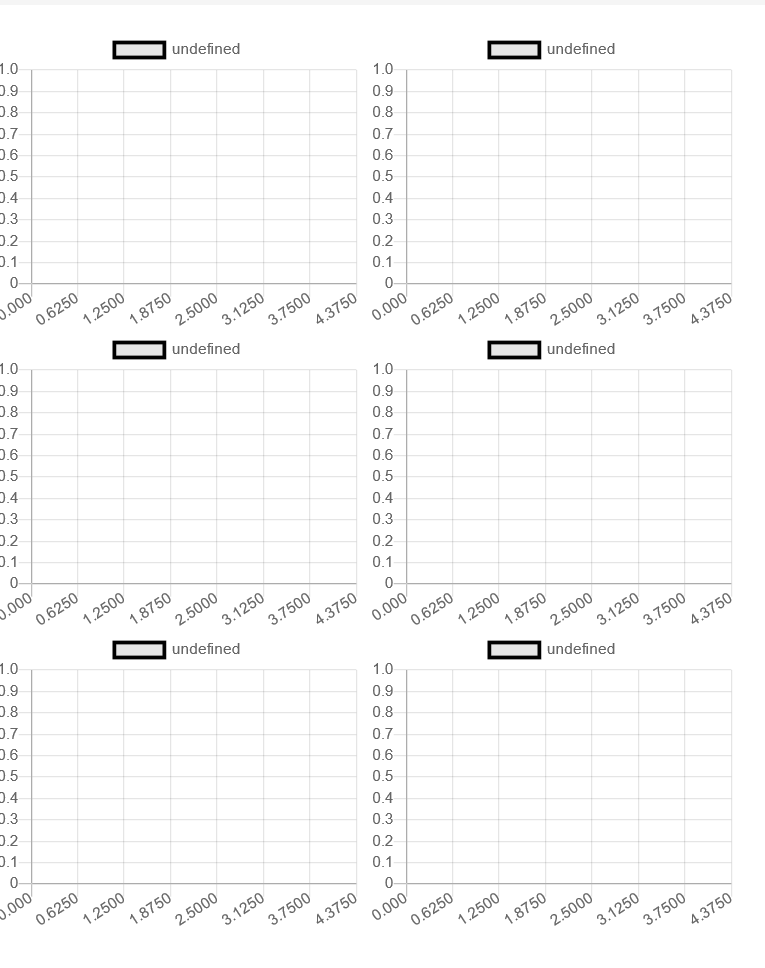
\includegraphics[width=0.80\textwidth]{pics/sixgraphsnoinit.PNG}
    \caption{Funktionsgraphen ohne Initialisierung}
    \label{fig:noinit}
\end{figure} 

Diese sechs Graphen werden zuerst ohne Daten nur mit ihren Labels erstellt und dann über die Methode \lstinline | loadChartData | befüllt.
LoadChartData wird über einen Button aufgerufen und mit einem weiteren Button können diese Graphen wieder geleert werden.
DataPoints und Labels wurden bereits in der Visualiserungskomponente [\ref{visualisation}] erläutert.
\begin{lstlisting}[language=Typescript, caption={Erstellen der Funktionsgraphen}]
  dataPointsBWA: ChartDataSets[] = [];
  BWALabels: Label[] = [ '0.000', '0.6250', '1.2500', '1.8750', '2.5000', '3.1250', '3.7500', '4.3750'];
  dataPointsBWB: ChartDataSets[] = [];
  BWBLabels: Label[] = [ '0.000', '0.6250', '1.2500', '1.8750', '2.5000', '3.1250', '3.7500', '4.3750'];
  dataPointsMWA: ChartDataSets[] = [];
  MWALabels: Label[] = [ '0.000', '0.6250', '1.2500', '1.8750', '2.5000', '3.1250', '3.7500', '4.3750'];
  dataPointsMWB: ChartDataSets[] = [];
  MWBLabels: Label[] = [ '0.000', '0.6250', '1.2500', '1.8750', '2.5000', '3.1250', '3.7500', '4.3750'];
  dataPointsRWA: ChartDataSets[] = [];
  RWALabels: Label[] = [ '0.000', '0.6250', '1.2500', '1.8750', '2.5000', '3.1250', '3.7500', '4.3750'];
  dataPointsRWB: ChartDataSets[] = [];
  RWBLabels: Label[] = [ '0.000', '0.6250', '1.2500', '1.8750', '2.5000', '3.1250', '3.7500', '4.3750'];
\end{lstlisting}

\begin{lstlisting}[language=Typescript, caption={Befüllen und Leeren der Funktionsgraphen}]
  loadChartData(){
    this.dataPointsBWA = [{data: [-30.0431, -29.0684, -28.7432, -28.2064, -27.8274, -27.9592, -25.7714, -28.1736], label: 'Lager Bremswelle A'}]
    this.dataPointsBWB = [{data: [-31.0431, -28.0684, -30.7432, -30.1064, -28.8274, -31.9592, -24.7714, -30.1736], label: 'Lager Bremswelle B'}]
    this.dataPointsMWA = [{data: [-27.0431, -28.0684, -30.7432, -27.1064, -30.8274, -29.9592, -24.7714, -31.1736], label: 'Lager Motorwelle A'}]
    this.dataPointsMWB = [{data: [-31.0431, -28.0684, -30.7432, -30.1064, -27.8274, -24.9592, -24.7714, -25.1736], label: 'Lager Motorwelle B'}]
    this.dataPointsRWA = [{data: [-28.0431, -28.0684, -31.7432, -27.1064, -24.8274, -29.9592, -24.7714, -30.1736], label: 'Lager Radwelle A'}]
    this.dataPointsRWB = [{data: [-31.0431, -28.0684, -30.7432, -30.1064, -27.8274, -30.9592, -28.7714, -25.1736], label: 'Lager Radwelle B'}]
  }


  clearCharts(){
    this.dataPointsBWA = [{data: [], label: ''}]
    this.dataPointsBWB = [{data: [], label: ''}]
    this.dataPointsMWA = [{data: [], label: ''}]
    this.dataPointsMWB = [{data: [], label: ''}]
    this.dataPointsRWA = [{data: [], label: ''}]
    this.dataPointsRWB = [{data: [], label: ''}]
  }
\end{lstlisting}

\begin{lstlisting}[language=HTML, caption={HTML-Code eines Funktionsgraphen}]
<div id="one" class="chartjs-block">
  <canvas baseChart height="240" width="300"
      [datasets]="dataPointsBWA"
      [labels]="BWALabels"
      [options]="options"
      [colors]="colors"
      [legend]="legend"
      [chartType]="type"
      [plugins]="plugins">
  </canvas>
</div>
\end{lstlisting} 

Der zuständige Prüfer kann über ein Dropdown-Menü ausgewählt werden, welches über Objekt-Binding mit dem selectedPruefer-Objekt der 
Typescript-Datei verbunden ist. 

\begin{lstlisting}[language=HTML, caption={HTML-Code des Dropdown-Menüs für den Prüfer}]
  <mat-form-field appearance="fill">
    <select matNativeControl [(ngModel)]="selectedPruefer" name="pruefer">
      <option value="" selected></option>
      <option *ngFor="let pruefer of pruefers" [value]="pruefer.p_nachname + ' ' + pruefer.p_vorname">
        {{pruefer.p_nachname}}
      </option>
    </select>
  </mat-form-field>
  <br/>
  Pruefer:
    <ng-template *ngIf="selectedPruefer.p_nachname === ''then one; else two"></ng-template>
    <ng-template #one></ng-template>
    <ng-template #two>{{selectedPruefer}}</ng-template>
\end{lstlisting}

Der Button Speichern ruft die Methode \lstinline | openDialog | auf, welche einen Dialog öffnet, in welchem ausgewählt werden kann, ob diese Prüfung
frei gegeben werden kann oder nicht und ob es zusätzliche Kriterien gibt, auf welche man achten muss.

\begin{lstlisting}[language=Typescript, caption={openDialog-Methode}]
  openDialog(): void{
    const dialogRef = this.dialog.open(DialogOverview, {
      width: '300',
      height: '500',
      data: {pruefer: this.selectedPruefer}
    });

    dialogRef.afterClosed().subscribe(result => {
      console.log('Pruefung wurde gespeichert');
    });
  }
\end{lstlisting}

Mit \lstinline|this.dialog.open| wird das Dialog-Fenster geöffnet, \lstinline | width | und \lstinline | heigth | geben die Dimensionen des Fensters an. Nachdem 
dieses Dialog-Fenster geschlossen wird, wird in der Konsole die Nachricht \dq Pruefung wurde gespeichert\dq ausgegeben. 

\begin{lstlisting}[language=Typescript, caption={TypeScript für DialogOverview}]
export class DialogOverview  {
  panelOpenState = false;
  kriterium = '';
  kriterien: String[] = [];

  constructor(
    public dialogRef: MatDialogRef<DialogOverview>,
    @Inject(MAT_DIALOG_DATA) public data: DialogData) {}

  onNoClick(): void {
    this.dialogRef.close();
  }
  save(): void{
    this.kriterien = [];
    this.dialogRef.close();
  }
  pushKriterium(): void{
    this.kriterien.push(this.kriterium);
    this.kriterium = '';
  }
}
\end{lstlisting}

\begin{lstlisting}[language=HTML, caption={HTML-Code für DialogOverview}]
<h1 mat-dialog-title>Pruefer: {{data.pruefer}}</h1>
<div mat-dialog-content>
  <mat-checkbox class="example-margin">Geprueft</mat-checkbox>&nbsp;
  <mat-checkbox class="example-margin">Geprueft und Frei</mat-checkbox>
</div>
<br/>
<div>
  <mat-accordion>
    <mat-expansion-panel hideToggle>
      <mat-expansion-panel-header>
        <mat-panel-title>
          Zusaetzliche Kriterien/Fehler
        </mat-panel-title>
      </mat-expansion-panel-header>
      <mat-list>
        <mat-list-item id="listitems" *ngFor="let item of kriterien" >
          <h3 matLine>{{item}}</h3>
        </mat-list-item>
      </mat-list>
      <mat-form-field class="example-full-width" appearance="fill">
        <input matInput value="" [(ngModel)]="kriterium">
      </mat-form-field>
      <button mat-icon-button (click)="pushKriterium()">
        <mat-icon>add</mat-icon>
      </button>
    </mat-expansion-panel>
  </mat-accordion>
</div>
<br/>
<div mat-dialog-actions>
  <button mat-button (click)="onNoClick()">Zurueck</button>
  <button mat-button (click)="save()">Speichern</button>
</div>
\end{lstlisting}

Über eine Checkbox kann der Status der Prüfung ausgewählt werden, geprüft oder geprüft und frei. Sollte es zusätzliche Kriterien 
geben, können diese in einem einfachen Textfeld eingegeben werden und über klicken auf den Plus-Button wird die Methode \lstinline | pushKriterium |
aufgerufen. Diese Methode fügt mit \lstinline | this.kriterien.push | das eingegebene Kriterium in ein vorher angelegtes Array von Kriterien hinzu
und leert das Textfeld dann wieder, um ein neues Kriterium angeben zu können. Mit einem Klick auf den Zurück-Button wird die Methode
\lstinline | onNoClick | aufgerufen, welche den Dialog wieder schließt und mit einem Klick auf den Speichern-Button wird die Methode \lstinline | save | aufgerufen,
welche den Dialog ebenfalls nur schließt, da dieses Mockup an keine Datenbank angebunden ist.